\section{半导体中的杂质}

\subsection{晶体中的间隙}
半导体的杂质,主要来源于制备半导体的原材料纯度不够,半导体单晶制备过程中及器件制造过程中的玷污,或是为了控制半导体的性质而人为掺入某种化学元素的原子。那么,现在的问题是,杂质进入半导体之后,它们分布在什么位置呢?下面以硅中的杂质为例说明。\cite{E1}\cite{S1}

硅是化学元素周期表中的第\Romnum{4}族元素,每个硅原子具有$4$个价电子,硅原子间以共价键方式结合形成晶体,呈金刚石构型,如\xref{fig:硅的晶体结构}所示。硅晶体的每个晶胞中包含$8$个原子,为便于后续讨论硅晶体中杂质的位置,我们将硅晶体的晶胞中的$8$个原子,依照其位置进行编号
\begin{enumerate}
    \item 位于晶胞角上的$1$个原子,编号为$C_1$
    \item 位于晶胞面上的$3$个原子,编号为$C_2,C_3,C_4$
    \item 位于晶胞内部的$4$个原子,编号为$C_5,C_6,C_7,C_8$
\end{enumerate}
在绘制晶胞时,由于边界的重复,会看起来有$6$个$C_1$和$C_2,C_3,C_4$各$2$个。

\begin{Figure}[硅的晶体结构]
    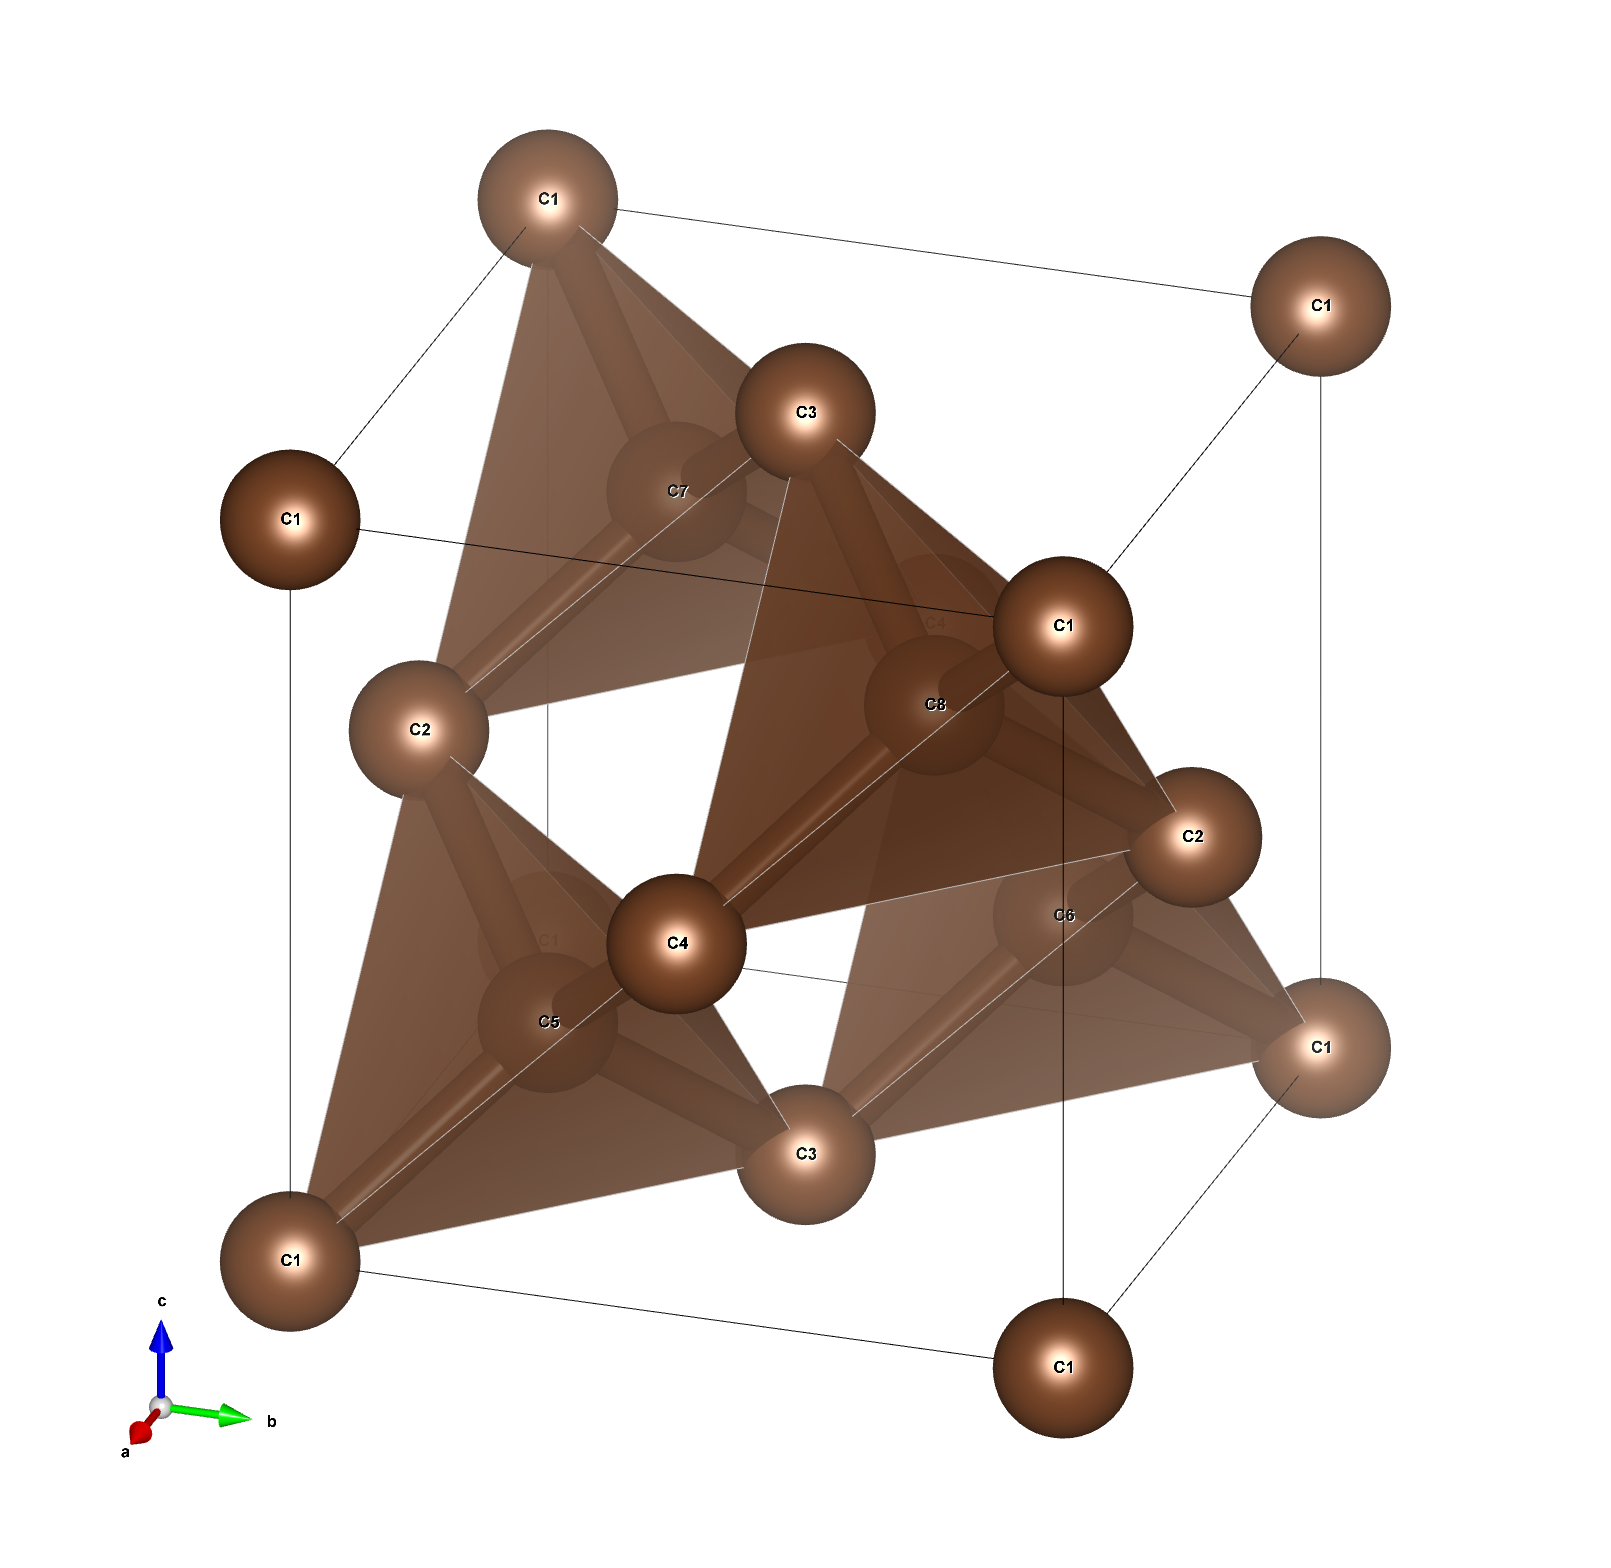
\includegraphics[width=5.8cm]{image/Diamond.png}
\end{Figure}

硅原子,若近似视为半径为$r$的圆球,那么是可以计算出锗$8$个原子占据晶胞空间的百分数的。硅原子在密积时,限制其半径的要素,是晶胞顶角的原子和距其$1/4$体对角线的内部原子间的距离,即,两倍原子半径应等于$1/4$体对角线,若半径为$r$而晶格常数为$a$,则
\begin{Equation}
    r=\frac{\sqrt{3}a}{8}
\end{Equation}
而$8$个硅原子的体积为
\begin{Equation}
    V=8\times\frac{4}{3}\pi r^3=\frac{\sqrt{3}}{16}a^3
\end{Equation}
而$8$个硅原子的体积与晶胞的体积比即为
\begin{Equation}
    V/V_a=\frac{\sqrt{3}}{16}=0.34
\end{Equation}
这表明,金刚石结构中,原子体积只占晶胞体积的$34\%$,换言之,原子间有很多空隙。

\begin{Figure}[硅的两类间隙]
    \begin{FigureSub}[四面体间隙]
        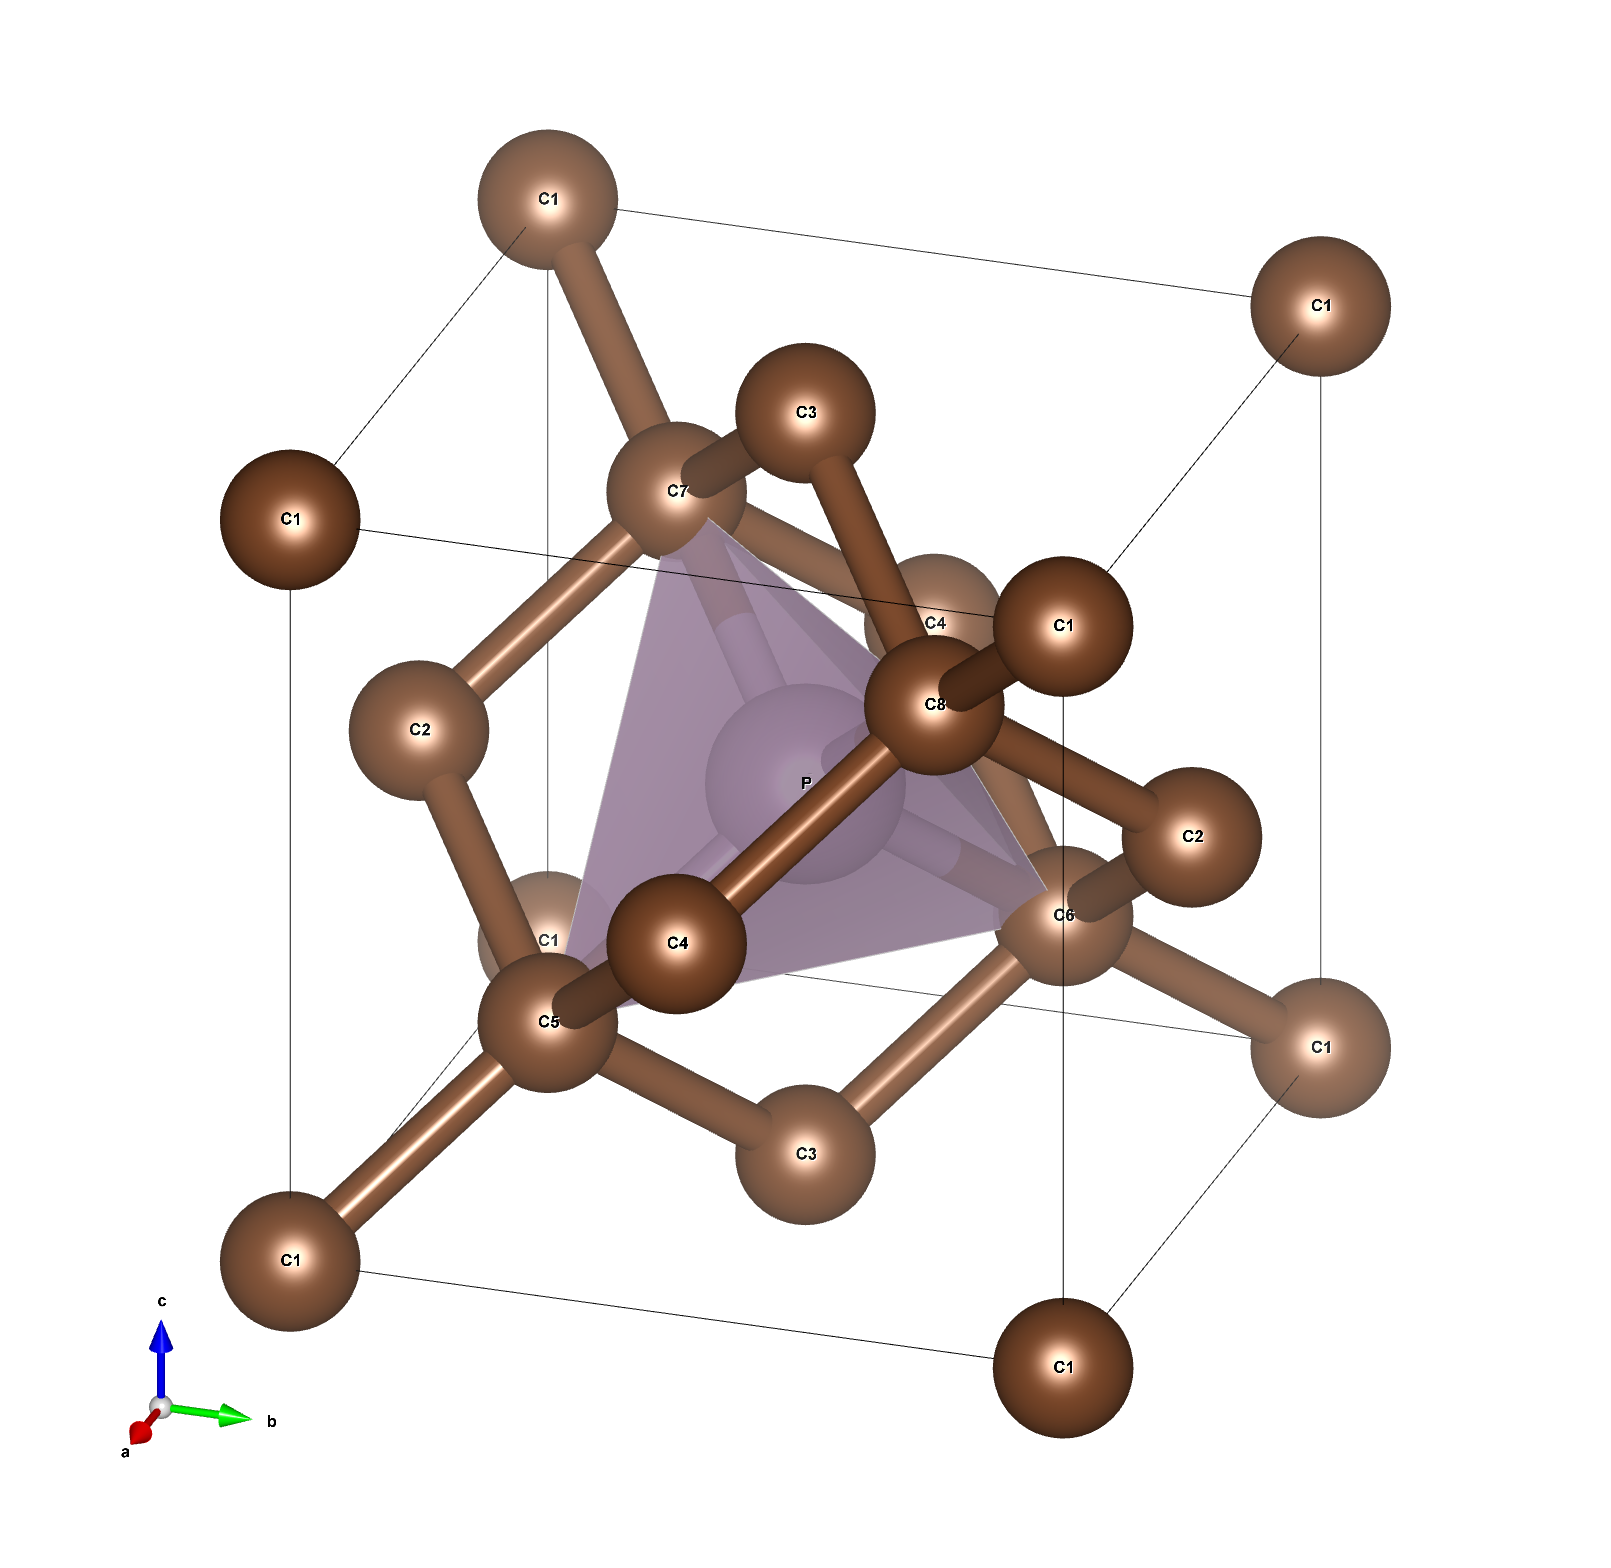
\includegraphics[width=5.8cm]{image/Diamond1.png}
    \end{FigureSub}
    \hspace{0.5cm}
    \begin{FigureSub}[六角形间隙]
        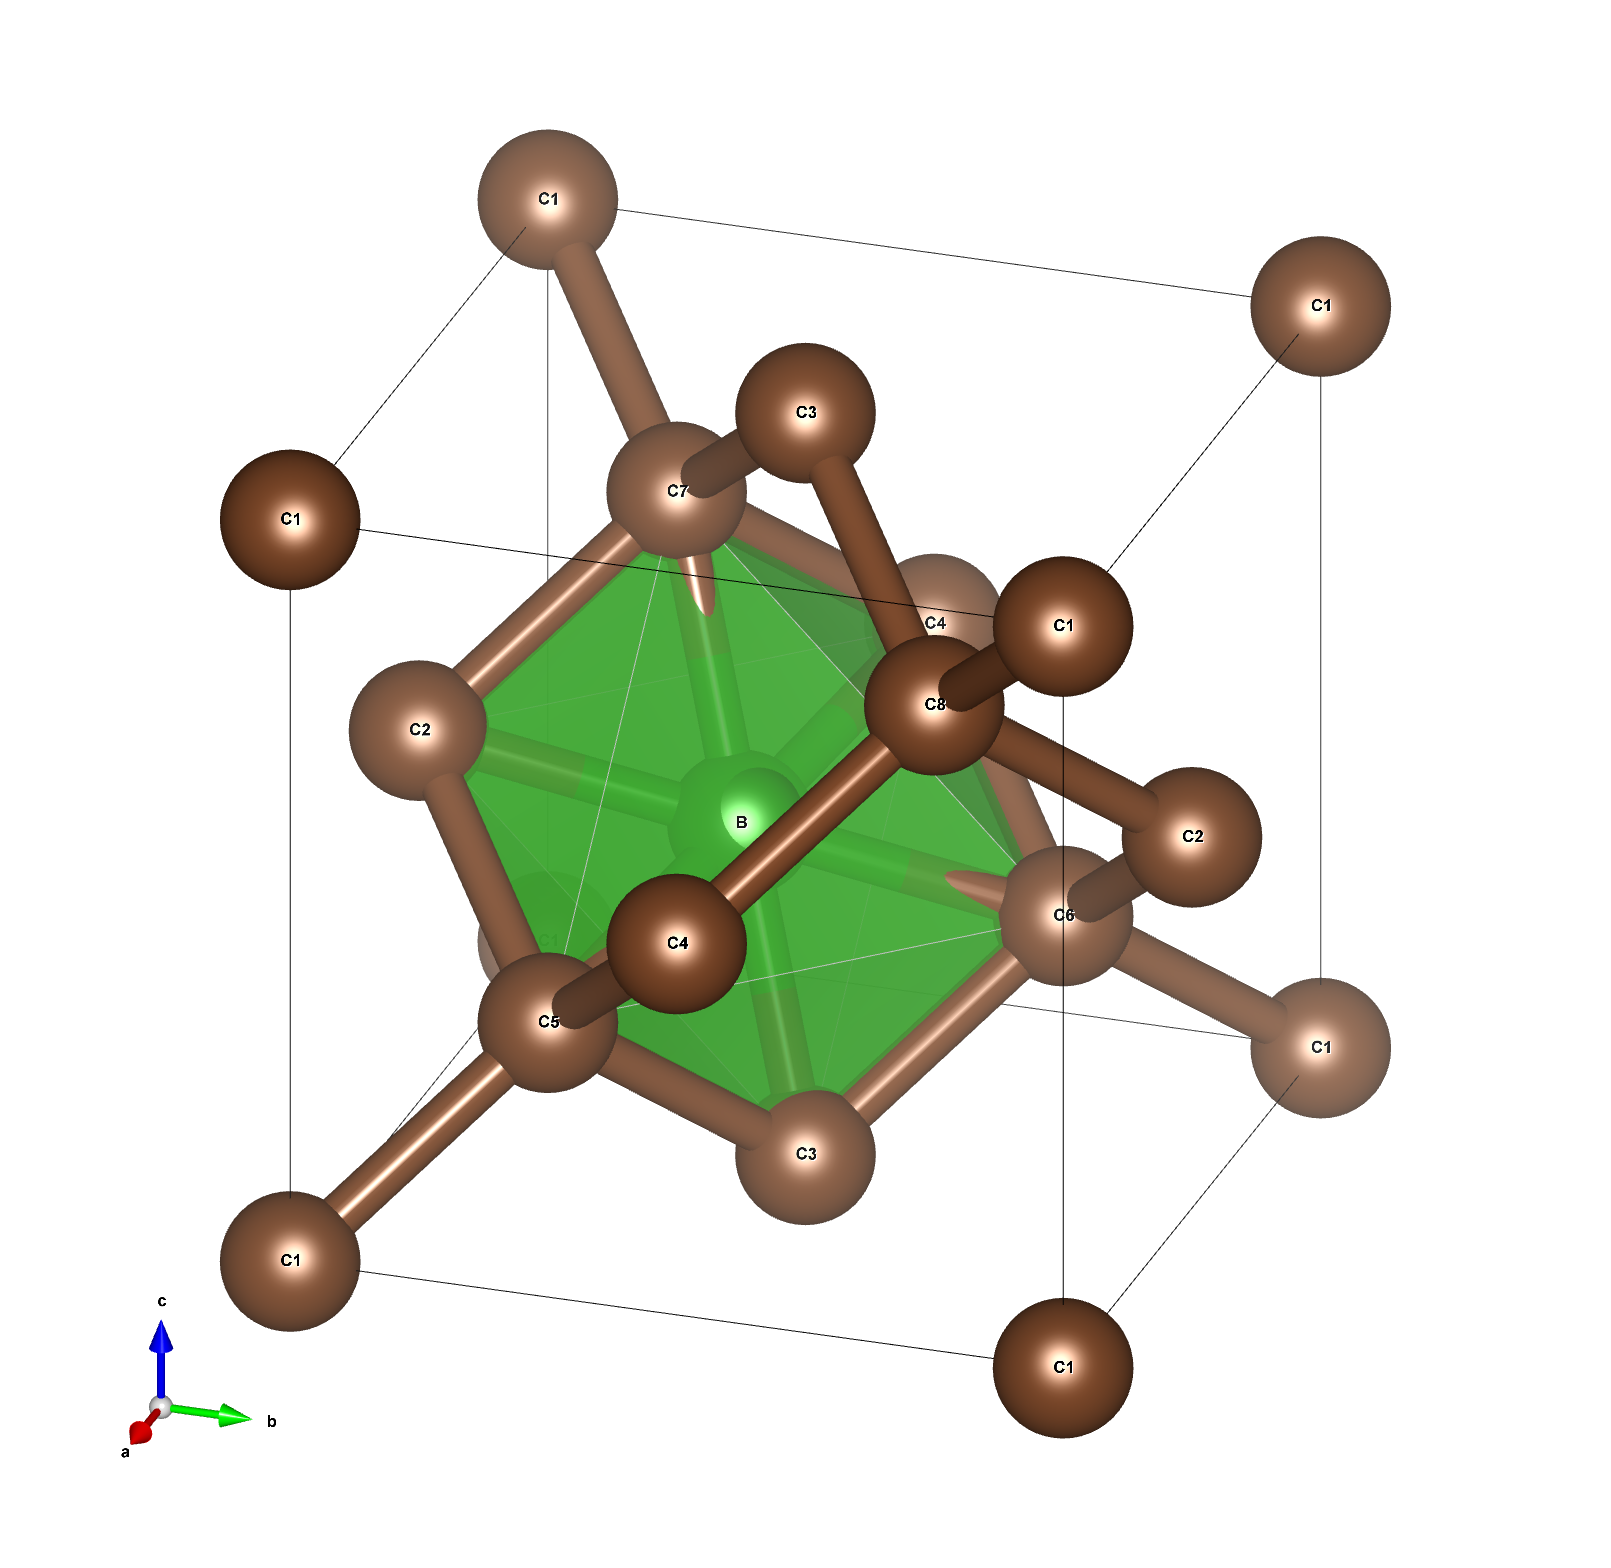
\includegraphics[width=5.8cm]{image/Diamond2.png}
    \end{FigureSub}
\end{Figure}

如\xref{fig:硅的两类间隙}所示\footnote{\xref{fig:硅的两类间隙}中的磷原子和硼原子仅为杂质示意,实际上这两者在硅中是以替位杂质而非间隙杂质的形态存在。},硅晶体中的间隙可以分为两类:\uwave{四面体间隙}、\uwave{六角形间隙}。\goodbreak

\begin{itemize}
    \item 四面体间隙是指,由四个内部原子$C_5,C_6,C_7,C_8$所构成的四面体中心。
    \item 六角形间隙是指,由四个内部原子$C_5,C_6,C_7,C_8$中的任意三个原子与相应三个面上的原子$C_2,C_3,C_4$构成的空间六边形的中心,该空间六边形有两层,由内部的三个原子和面上的三个原子分别构成了两个相错$60^{\circ}$且相隔一定距离的两个等边三角形组成。
\end{itemize}
在\xref{fig:金刚石结构中的空间六角形}中我们通过一个特别的角度观察\xref{fig:硅的晶体结构},就可以很直观的看到空间六边形
\begin{Figure}[金刚石结构中的空间六角形]
    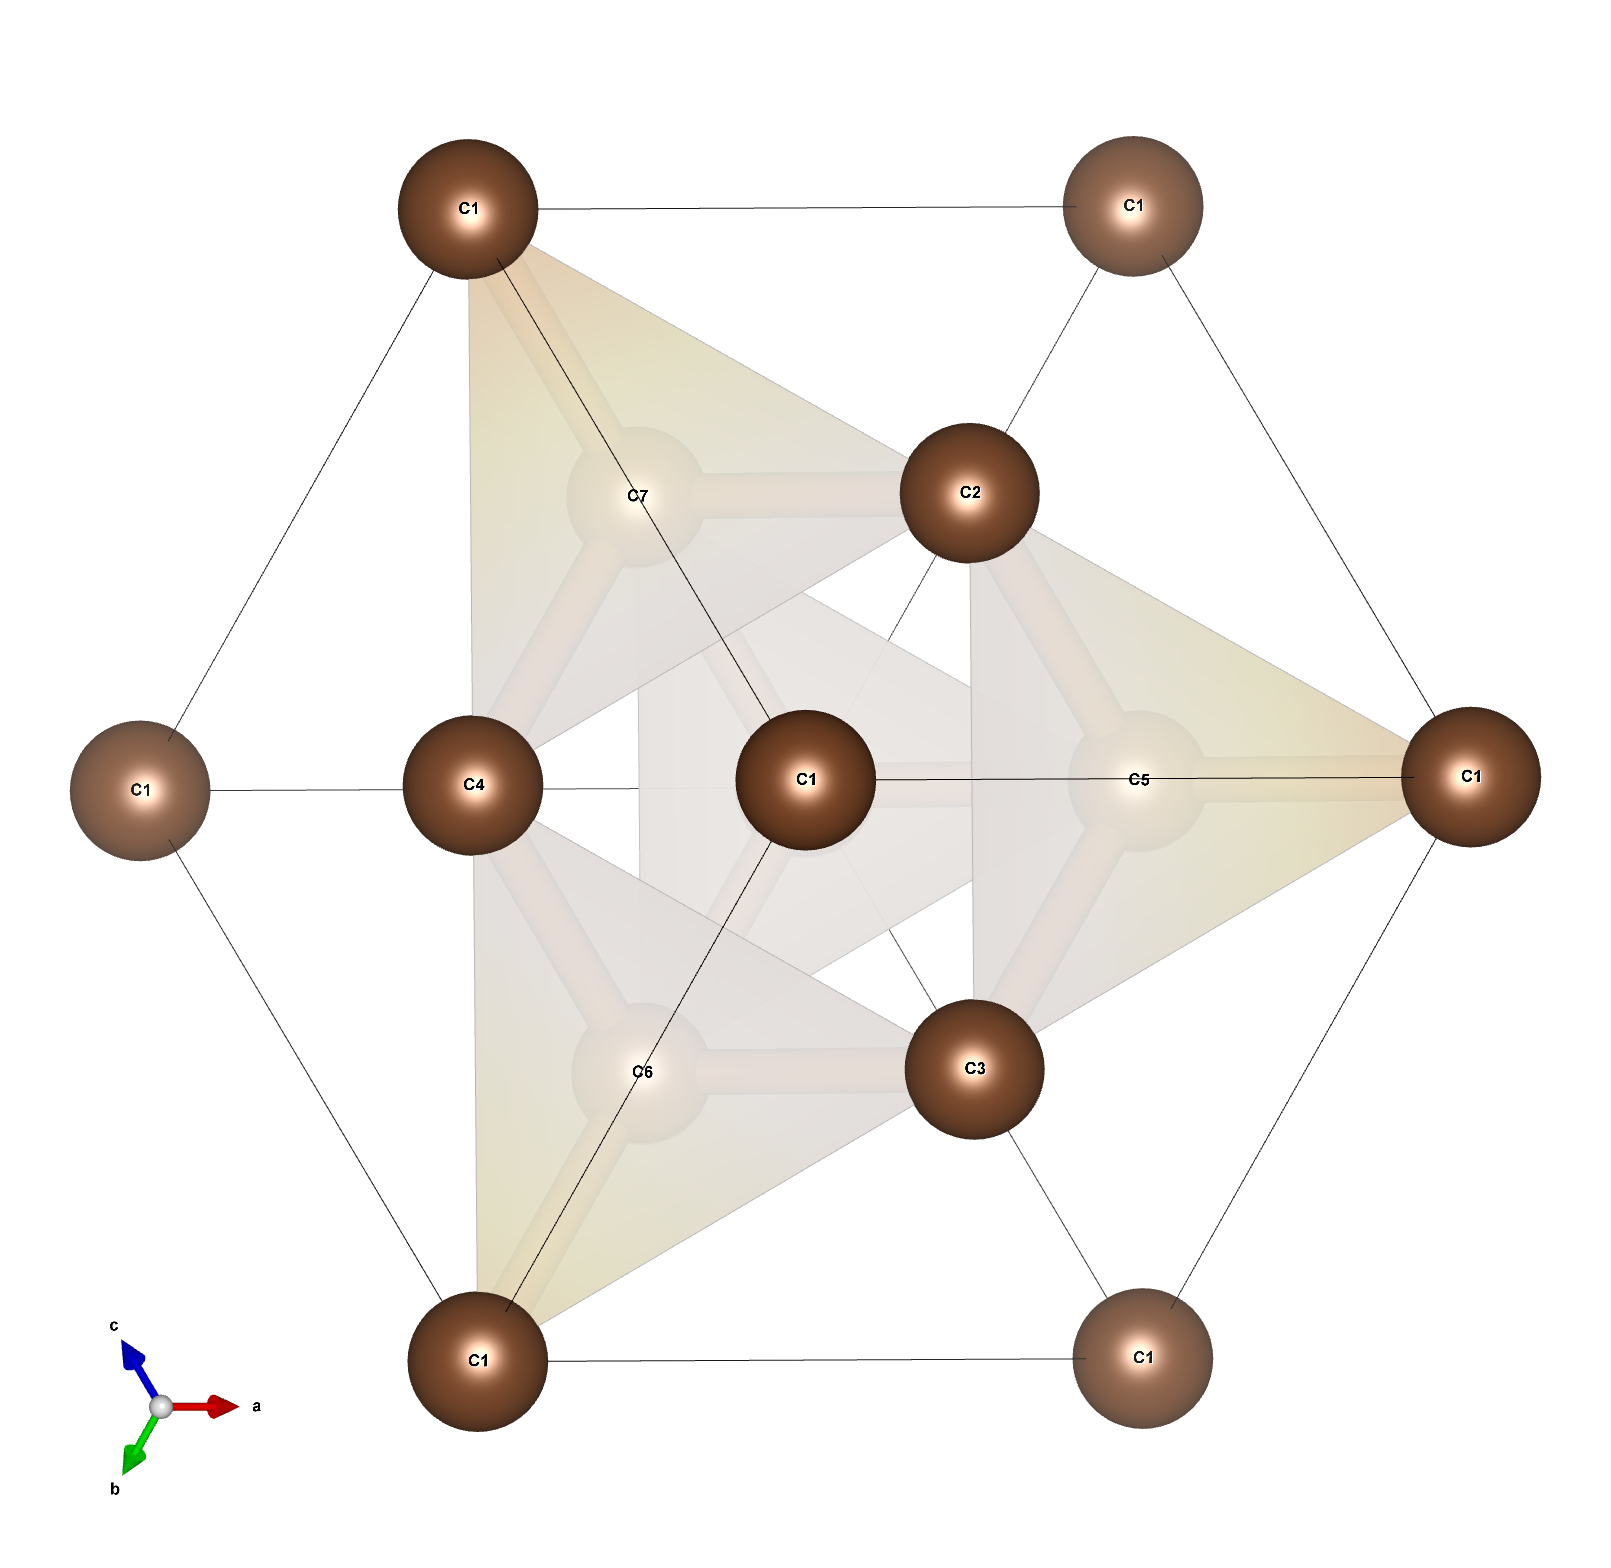
\includegraphics[width=5.5cm]{image/Diamond_HEX.png}
\end{Figure}

\subsection{间隙杂质和替位杂质}

实际上,当杂质原子进入半导体材料后,只可能以两种方式存在
\begin{enumerate}
    \item 杂质原子占据晶格原子间的间隙位置,称为\uwave{间隙式杂质}(Interstitial Impurity)。
    \item 杂质原子取代晶格原有的原子,位于格点,称为\uwave{替位式杂质}(Substitution Impurities)。
\end{enumerate}
间隙式杂质要求杂质原子体积较小,替位式杂质要求杂质原子与晶格原有的原子体积相近,并且还要求它们的价电子壳层结构比较相近。在硅和锗晶体中,通常只有离子锂可以形成间隙式杂质,而通常掺杂的\Romnum{3}族和\Romnum{5}族元素(磷、硼)其实都是以替位式杂质的形态存在的。

\subsection{施主杂质和受主杂质}
我们知道,\Romnum{3}族和\Romnum{5}族元素在硅和锗中是替位式杂质
\begin{itemize}
    \item 磷原子(\hspace{0.35em}\Romnum{5}\hspace{0.35em}族元素)有$5$个价电子,其在与周围的硅原子形成共价键后,还多了一个价电子,如\xref{fig:施主杂质}。故掺杂\hspace{0.5em}\Romnum{5}\hspace{0.5em}族元素将引入电子,称为\uwave{施主杂质}(Donor Impurity)。
    \item 硼原子(\Romnum{3}族元素)有$3$个价电子,其在与周围的硅原子形成共价键后,还少了一个价电子,如\xref{fig:受主杂质}。故掺杂\Romnum{3}族元素将引入空穴,称为\uwave{受主杂质}(Acceptor Impurity)。
\end{itemize}
我们说,杂质引入的电子或空穴最初都是被束缚在相应的杂质原子旁的,但是,这种束缚作用要比共价键弱很多,只需要很少的能量就能使电子和空穴摆脱杂质原子的束缚,形成可以在晶体中自由运动的导电电子或导电空穴,并在原位留下不能移动的正电中心或负电中心。该过程还称为\uwave{杂质电离}(Impurity Ionization),所需的能量称为\uwave{杂质电离能}(Impurity Ionization Energy),电离前中性的杂质原子称为\uwave{中性态}或\uwave{束缚态},电离后的杂质原子则称为\uwave{离化态}。
\begin{Figure}[施主杂质和受主杂质]
    \begin{FigureSub}[施主杂质]
        \includegraphics[scale=0.75]{build/Chapter02A_02.fig.pdf}
    \end{FigureSub}
    \hspace{1cm}
    \begin{FigureSub}[受主杂质]
        \includegraphics[scale=0.75]{build/Chapter02A_01.fig.pdf}
    \end{FigureSub}
\end{Figure}

\begin{itemize}
    \item 施主杂质的电离,称为\uwave{施主电离},而相应的电离能记为$\delt{E_\text{D}}$,即当电子得到能量$\delt{E_\text{D}}$后,就能从施主的束缚态跃迁到导带称为导带电子。因此电子被施主杂质束缚时的能量比导带底$E_\text{c}$低$\delt{E_\text{D}}$,将被施主杂质束缚的电子的能量状态称为施主能级,以$E_\text{D}$标识。
    \item 受主杂质的电离,称为\uwave{受主电离},而相应的电离能记为$\delt{E_\text{A}}$,即当空穴得到能量$\delt{E_\text{A}}$后,就能从受主的束缚态跃迁到价带称为价带空穴。因此空穴被受主杂质束缚时的能量比价带底$E_\text{v}$低$\delt{E_\text{A}}$,将被施主杂质束缚的电子的能量状态称为受主能级,以$E_\text{A}$标识。
\end{itemize}

施主能级和受主能级可以在能带图上标注,如\xref{fig:施主能级和受主能级}所示,我们用一系列的短线段表示施主能级$E_\text{D}$和受主能级$E_\text{A}$,每一条短线段代表一个杂质原子,以凸显施主能级和受主能级是一些具有相同能量的孤立能级(能量之所以相同,是因为杂质原子很少,从而可以忽略杂质原子间的相互作用)。除此之外,我们还用$\oplus$和$\ominus$表示杂质原子电离后的正电中心和负电中心。
\begin{Figure}[施主能级和受主能级]
    \begin{FigureSub}[施主能级]
        \includegraphics[scale=0.65]{build/Chapter02A_03.fig.pdf}
    \end{FigureSub}
    \hspace{1cm}
    \begin{FigureSub}[受主能级]
        \includegraphics[scale=0.65]{build/Chapter02A_04.fig.pdf}
    \end{FigureSub}
\end{Figure}

这里需要说明的是,在能带图中,电子的能量是越向上越高,空穴的能量是越向下越高,这就是为什么我们前面说$E_\text{A}$比$E_\text{v}$低$\delt{E_\text{A}}$,但能带图中$E_\text{A}$却比$E_\text{v}$高的原因。事实上,受主电离的实质仍然是电子的运动,是价带中的电子得到能量$\delt{E_\text{A}}$跃迁到受主能级,并与被束缚在受主能级上的空穴复合,同时在价带上留下了一个新的空穴,这样来理解就比较通顺了。

我们知道,在纯净半导体中,同时有导带电子和价带空穴进行导电,但是,纯净半导体中的载流子完全来自本征激发,数量很少,因此掺入杂质后,载流子就主要取决于杂质的类型了
\begin{itemize}
    \item 在半导体中掺入施主杂质将向导带引入大量电子,称为\uwave{N型半导体}。
    \item 在半导体中掺入受主杂质将向价带引入大量空穴,称为\uwave{P型半导体}。
\end{itemize}

我们在此总结一下,\Romnum{5}族元素和\Romnum{3}族元素在硅和锗晶体中分别是施主杂质和受主杂质,它们在禁带中引入能级,施主能级$E_\text{D}$比导带底低$\delt{E_\text{D}}$,受主能级$E_\text{A}$比价带顶高$\delt{E_\text{A}}$(统一使用电子视角),电离后,施主原子产生电子和正点中心,受主原子产生空穴和负电中心,电子和空穴分别进入导带和价带参与导电。实验证明,硅和锗中的\Romnum{5}族和\Romnum{3}族杂质的电离能都很小,因此,施主能级很接近导带底,受主能级很接近价带顶。我们通常将这些杂质称为称为\uwave{浅能级杂质}(Shallow Impurity),对应\uwave{深能级杂质}(Deep Impurity)。另外,在室温下,晶格原子振动的能量传递给电子,就足矣使得硅和锗中的\Romnum{5}族和\Romnum{3}族杂质原子几乎全部离化。

最后,我们列出部分\Romnum{5}族元素和\Romnum{3}族元素在硅和锗中的电离能\cite{B2}
\begin{Table}[部分杂质的电离能]{llllllll}
<\mr{2}{半导体}&\mc{3}(c){施主杂质/$\delt{E_\text{D}},\si{eV}$}&\mc{4}(c){受主杂质/$\delt{E_\text{A}},\si{eV}$}\\
&
\mc{1}(c){磷\xce{P}}&
\mc{1}(c){砷\xce{As}}&
\mc{1}(c){锑\xce{Sb}}&
\mc{1}(c){硼\xce{B}}&
\mc{1}(c){铝\xce{Al}}&
\mc{1}(c){镓\xce{Ga}}&
\mc{1}(c){铟\xce{In}}\\>
硅\xce{Si}&
0.045&0.053&0.043&0.046&0.067&0.071&0.154\\
锗\xce{Ge}&
0.0120&0.0127&0.0096&0.0104&0.0102&0.0108&0.0112\\
\end{Table}
由\xref{tab:部分杂质的电离能}可见,\Romnum{5}族元素和\Romnum{3}族元素在硅和锗中的电离能都不大,无论是施主杂质还是受主杂质,硅中电离能普遍在$0.05\si{eV}$(铟的$0.154\si{eV}$是特例),锗中电离能普遍在$0.01\si{eV}$。

\subsection{杂质的补偿作用}
假如在半导体中,同时存在着施主杂质和受主杂质,半导体究竟是N型还是P型呢?形象的说,这其实就是一个“水多了加面,面多了加水”的过程,关键取决于哪种杂质比较多,因为施主杂质和受主杂质之间具有相互抵消的作用。我们将这种相互作用称为\uwave{杂质的补偿作用}。

实际上,无论是施主杂质和受主杂质哪一方比较多,补偿作用的效果都是一致的,即施主能级的电子会跃迁至能级更低的受主能级并与其上的空穴复合,如\xref{fig:杂质的补偿作用}所示,而在此基础上
\begin{itemize}
    \item 若施主杂质掺杂量远高于受主杂质,即$N_\text{D}\gg N_\text{A}$,经过中和后,在施主能级上仍然剩有$N_\text{D}-N_\text{A}$个电子,可以跃迁至导带形成导带电子,故此时表现为N型半导体。
    \item 若施主杂质掺杂量远高于受主杂质,即$N_\text{D}\ll N_\text{A}$,经过中和后,在受主能级上仍然剩有$N_\text{A}-N_\text{D}$个空穴,可以跃迁至价带形成价带空穴,故此时表现为P型半导体。
\end{itemize}

很明显,补偿作用并不利于杂质半导体性质,那为什么我们要这样做呢?因为制造半导体器件的过程中,我们往往会使用N型或P型衬底材料,在此基础上,在局部通过扩散或离散注入的方式,以改变某一区域的导电类型,制成各种半导体器件,所以,补偿作用是不可避免的。

\begin{Figure}[杂质的补偿作用]
    \begin{FigureSub}[施主杂质多于受主杂质]
        \includegraphics[scale=0.65]{build/Chapter02A_05.fig.pdf}
    \end{FigureSub}
    \hspace{1cm}
    \begin{FigureSub}[受主杂质多于施主杂质]
        \includegraphics[scale=0.65]{build/Chapter02A_06.fig.pdf}
    \end{FigureSub}
\end{Figure}

但是,如果该过程中控制不当,可能会出现$N_\text{D}\approx N_\text{A}$的情况,此时中和后,施主能级上没有更多的电子,受主能级上没有更多的空穴,虽然杂质很多,但不能像导带和价带提供电子和空穴,这种现象称为杂质的高度补偿,这种该材料很容易被误认为是高纯半导体,但实际上杂质很多,性能很差,是无法使用的(形象的说,反复加水加面的面团,最后只能弃之不用)。

\subsection{浅能级杂质}
上述提到的杂质(硅和锗中掺入\Romnum{5}族或\Romnum{3}族元素)都是浅能级杂质,电离能都很低,电子或空穴受到正电中心或负电中心的束缚很微弱,可以利用类氢模型来估算杂质的电离能,我们不妨这样想,正电中心就是氢原子核,正电中心电离产生的电子就是氢原子的核外电子。

根据大学物理中氢原子的波尔模型,能级$E_n$是
\begin{Equation}
    E_n=-\frac{m_0q^4}{2(4\pi\varepsilon_0)^2\hbar^2n^2}
\end{Equation}
取$n=1$即得$-13.6\si{eV}$的基态能量
\begin{Equation}
    E_1=-\frac{m_0q^4}{2(4\pi\varepsilon_0)^2\hbar^2}=-13.6\si{eV}
\end{Equation}
容易注意到当$n\to\infty$时有$E_n\to 0$,而$E_{\infty}$就是电子完全摆脱氢原子对应的能级。

因此,氢原子电子的电离能即为
\begin{Equation}
    \delt{E}=E_{\infty}-E_{1}=\frac{m_0q^4}{2(4\pi\varepsilon_0)^2\hbar^2}
\end{Equation}
而这里将氢原子模型用于杂质电离能的计算时,要作两点改变,首先考虑到周期性势场的影响,需要将电子质量$m_0$更换为相应的有效质量$\mne$或$\mpe$,取决于是电子还是空穴。其次考虑到硅和锗作为电介质,我们需要将$\varepsilon_0$替换为$\varepsilon_0\varepsilon_r$,其中,硅的$\varepsilon_r=12$,锗的$\varepsilon_r=16$。

\begin{BoxFormula}[施主杂质的电离能]
    施主杂质的电离能可以表示为
    \begin{Equation}
        \delt{E_\text{D}}=\frac{\mne q^4}{2(4\pi\varepsilon\varepsilon_r)^2\hbar^2}=\frac{\mne}{m_0}\frac{E_0}{\varepsilon_r^2}
    \end{Equation}
\end{BoxFormula}

\begin{BoxFormula}[受主杂质的电离能]
    受主杂质的电离能可以表示为
    \begin{Equation}
        \delt{E_\text{A}}=\frac{\mpe q^4}{2(4\pi\varepsilon\varepsilon_r)^2\hbar^2}=\frac{\mpe}{m_0}\frac{E_0}{\varepsilon_r^2}
    \end{Equation}
\end{BoxFormula}

基于氢原子模型的杂质电离能的计算精度并不高,只能作为数量级上的估算,因为其根本没有考虑杂质原子类型的影响,所有杂质原子对其而言都是完全相同的正电中心或负电中心。

\subsection{深能级杂质}
在半导体硅和锗中,除了\Romnum{3}族和\Romnum{5}族杂质产生浅能级外,如果我们将其他各族元素掺入硅和锗中,情况又会怎么样呢?大量实验结果表明,它们也能在禁带中产生能级,有以下特点
\begin{enumerate}
    \item 由非\Romnum{3},\Romnum{5}族杂质产生的能级,施主能级距导带底较远,受主能级距价带顶较远,有时甚至可能倒挂\footnote{就是说,施主能级反而更靠近价带顶,受主能级反而更靠近导带底。},这种杂质能级被形象的称为深能级,区别于\Romnum{3},\Romnum{5}族形成的浅能级。
    \item 由非\Romnum{3},\Romnum{5}族杂质产生的能级,往往会通过多次电离或复合引入若干个杂质能级,而且有些杂质,既能引入施主能级,又能引入受主能级。例如金原子\xce{Au}中仅包含了一个价电子,其作为硅和锗中的杂质时,即可以电离出这个电子形成正电中心\xce{Au+},产生一个极深的施主能级$E_\text{D}$,也可以接受$1,2,3$个电子,形成负电中心\xce{Au-, Au^{2-}, Au^{3-}},由于随着接受电子数量的增加,电子间库伦排斥力逐渐增大,这将产生三个由浅到深的受主能级$E_\text{A1},E_\text{A2},E_\text{A3}$(不过即便$E_\text{A1}$也算深能级了),金原子的四个能级间的关系是
\end{enumerate}
\begin{Equation}
    E_\text{D}<E_\text{A1}<E_\text{A2}<E_\text{A3}
\end{Equation}
金是一种很典型的复合中心,在制造高速开关器件,常有意掺入金以提高器件速度。